\chapter{Recurrent Neural Networks}
\textbf{Recurrent Neural Networks} (RNN) are a family of neural networks for
processing sequential data. It is specialized for processing sequence of values
$x^{(1)}, \dots, x^{(\tau)}$. Recurrent networks can scale to much longer sequences
than would be practical for networks without sequence-based specialization. Most
recurrent networks can also process sequences of variable length.

To go from multilayer networks to recurrent networks, we need to take advantage
of one of the early ideas: sharing parameters across different parts of a model.
Parameter sharing makes it possible to extend and apply the model to examples of
different forms (different lengths, here) and generalize across them.

Recurrent networks share parameters differently compared to CNNs. Each output
member is a function of the previous output members and is produced using the
same update rule applied recursively to the earlier outputs. This recurrent
formulation leads to parameter sharing across a very deep computational graph.

Usually, RNN are defined using computational graph (CG) (Figure \ref{fig:rnn}).
In particular, in the Figure \ref{fig:rnn} we used the following notation:
\begin{itemize}
    \item $x^{(i)}$ is a value of the input sequence;
    \item $h^{(i)}$ represent the hidden layers;
    \item $o^{(i)}$ represent the output layer;
    \item $y^{(i)}$ represent the training target;
    \item $L^{(i)}$ is the loss that measures how far each $o$ is from the
          corresponding training target $y$.
\end{itemize}
The RNN has input-to-hidden connections parametrized by a weight matrix $\textbf{U}$,
hidden-to-hidden recurrent connections parametrized by a weight matrix $\textbf{W}$,
and hidden-to-output connections parametrized by a weight matrix $\textbf{V}$.

RNN uses the information coming from previous hidden layers to compute actual
prevision. There are also variants whose only occurrence is the feedback link
from the output to the hidden layer (Figure \ref{fig:rnn1}). This mechanism
implements \textbf{memory} behaviors.


This architecture is designed to apply the same operations to all the data of the
sequence. All inputs and outputs are dependent, because we apply the same operation
on all data using past operations.

There are different architectures of RNN:
\begin{itemize}
    \item RNNs that produces output for each time step and the recurrent connection
          from the previous hidden layer to the next hidden layer. (Figure \ref{fig:rnn})
    \item RNN that produces output for each time step and the recurrent connection
          is from output to the next hidden layer. (Figure \ref{fig:rnn1})
    \item RNN that doesn't produce output for each time step, but we have the
          recurrent connection from output to the next hidden layer. At the end
          of the sequence we produce output. (Figure \ref{fig:rnn2})
\end{itemize}

\begin{figure}[!ht]
    \centering
    \begin{subfigure}[b]{0.3\textwidth}
        \centering
        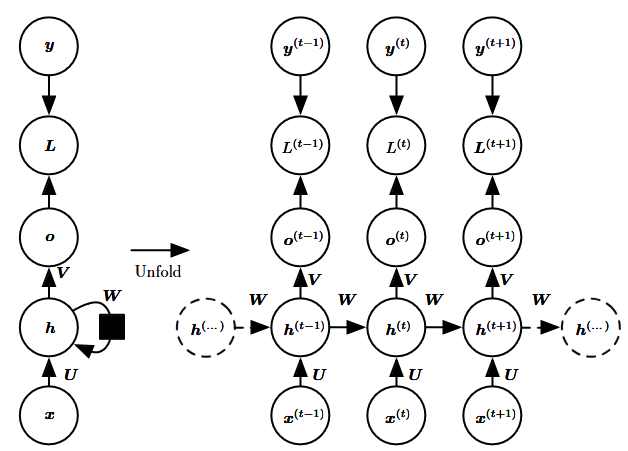
\includegraphics[width=\linewidth]{img/RNN/RNN.png}
        \caption{The computational graph of a recurrent network}
        \label{fig:rnn}
    \end{subfigure}
    \hfill
    \begin{subfigure}[b]{0.3\textwidth}
        \centering
        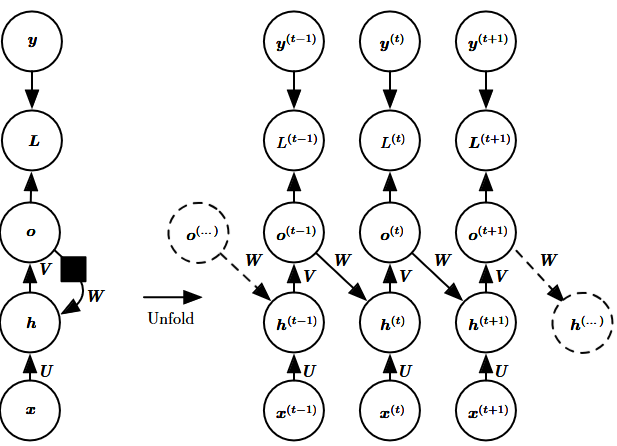
\includegraphics[width=\linewidth]{img/RNN/RNN1.png}
        \caption{An RNN whose only recurrence is the feedback connection from the
            output to the hidden layer.}
        \label{fig:rnn1}
    \end{subfigure}
    \hfill
    \begin{subfigure}[b]{0.3\textwidth}
        \centering
        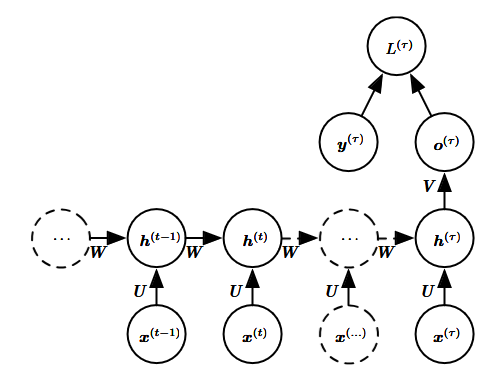
\includegraphics[width=\linewidth]{img/RNN/RNN2.png}
        \caption{Recurrent neural network with a single output at the end of the sequence}
        \label{fig:rnn2}
    \end{subfigure}
\end{figure}

The use of multiple layers in various parts of an RNN—input, hidden, and output
layers—can enhance performance; however, there is currently no theoretical proof
to support this.

To train such models, we can apply a similar approach to the architectures discussed
previously. However, some adjustments are necessary, as the information is derived
not only from the input layers but also from past hidden layers.

Computing the gradient of this loss function with respect to the parameters is an
expensive operation. The gradient computation involves performing a forward
propagation pass moving left to right through our illustration of the unrolled
graph, followed by a backward propagation pass moving right to left through
the graph. The runtime is $\mathcal{O}(\tau)$ and cannot be reduced by parallelization
because the forward propagation graph is inherently sequential; each time step
may be computed only after the previous one. States computed in the forward pass
must be stored until they are reused during the backward pass, so the memory cost
is also $\mathcal{O}(\tau)$. The back-propagation algorithm applied to the unrolled
graph with $\mathcal{O}(\tau)$ cost is called \textbf{back-propagation through time} (BPTT).

For notation purposes let's use $o^{(t)} =  \hat{y}^{(t)}$ Then consider:
\begin{equation}
    h^{(t)} = \tanh (U \cdot x^{(t)} + W \cdot h^{(t - 1)}) \,\, \land \,\, \hat{y}^{(t)} = softmax(V \cdot h^{(t)})
\end{equation}
And the cross entropy as the loss (i.e., error) function to minimize:
\begin{equation}
    E(y, \hat{y}) = \sum_t E^{(t)}(y^{(t)}, \hat{y}^{(t)}) = - \sum_t y^{(t)} \cdot \log(\hat{y}^{(t)})
\end{equation}

The goal of BPTT is to calculate the gradients of the error with reference to
$U, V, W$ and then learn good values of these parameters using Stochastic Gradient
Descent. Just like we sum up the errors, we also sum up the gradients at each
time step for one training example:
\begin{equation}
    \frac{\partial E}{\partial U} = \sum_t \frac{\partial E^{(t)}}{\partial U}, \,\, \land \,\,
    \frac{\partial E}{\partial V} = \sum_t \frac{\partial E^{(t)}}{\partial V}, \,\, \land \,\,
    \frac{\partial E}{\partial W} = \sum_t \frac{\partial E^{(t)}}{\partial W}
\end{equation}

To calculate these gradients, we use the differentiation chain rule, which
underpins the (traditional) backpropagation algorithm. While the computation of
$\frac{\partial E}{\partial V}$ may be relatively straightforward depending on
the RNN architecture, applying the chain rule to compute $\frac{\partial E}{\partial U}$
and $\frac{\partial E}{\partial W}$ is much more complex. This is because we must
backpropagate the gradients from the output, through the network, and all the way
back to $t = 0$.

The basic problem is that gradients propagated over many stages tend to either
\textbf{vanish} (most of the time) or \textbf{explode} (rarely, but with much
damage to the optimization). The difficulty with long-term dependencies arises
from the exponentially smaller weights given to long-term interactions (involving
the multiplication of many matrices) compared to short-term ones.

One might hope to avoid the problem by staying in a region of parameter space where
gradients neither vanish nor explode. Unfortunately, for the RNN to store memories
in a manner robust to small perturbations, it must enter a region of parameter
space where gradients vanish. Specifically, whenever the model can represent
long-term dependencies, the gradient of a long-term interaction has an exponentially
smaller magnitude compared to the gradient of a short-term interaction. This does
not mean it is impossible to learn long-term dependencies, but rather that it
might take a very long time, as the signal associated with these dependencies is
often overshadowed by the smallest fluctuations arising from short-term dependencies.

Since we need to compute a product of gradients at each time step, we may encounter
one of the following issues:
\begin{itemize}
    \item \textbf{Exploding gradients}: This occurs when all gradients are $> 1$.
          It can be mitigated by gradient clipping;
    \item \textbf{Vanishing gradients}: This arises when all gradients are $< 1$,
          leading to challenges in training. Solutions include using appropriate
          activation functions, weight initialization strategies, or modifying
          the network architecture, with the latter being the most effective
          approach for addressing vanishing gradients.
\end{itemize}

Solutions to the vanishing gradient problem are typically implemented as follows:
\begin{itemize}
    \item \textbf{Activation functions}: ReLU is preferred over tanh or sigmoid,
          as it mitigates vanishing gradients more effectively. (Figure \ref{fig:activation})
          \begin{figure}[!ht]
              \centering
              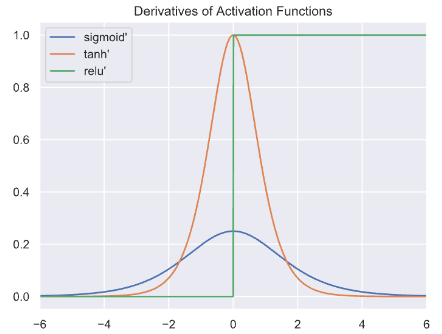
\includegraphics[width=0.3\linewidth]{img/RNN/derivatives.png}
              \caption{Solution 1: Activation function. ReLU prevents $f'$, to
                  shrink gradients when $x > 0$}
              \label{fig:activation}
          \end{figure}
    \item \textbf{Initialization}: We can initialize weights as an identity matrix
          and biases as 0, though this approach is not universally effective.
    \item \textbf{Architecture}: Modifying the architecture by incorporating gates
          to regulate the flow of information (e.g., as seen in ResNet) often
          proves to be the most robust solution.
\end{itemize}
\section{Gated RNNs}
In standard RNNs Figure \ref{fig:sRNN}, repeating modules contain a simple
computation node.
\begin{figure}[!ht]
    \centering
    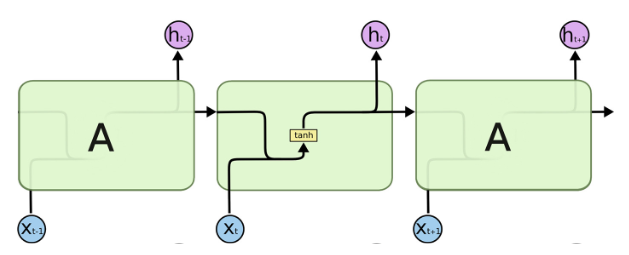
\includegraphics[width=0.5\linewidth]{img/RNN/sRNN.png}
    \caption{Standard RNN representation}
    \label{fig:sRNN}
\end{figure}

The most effective sequence models used in practical applications are called
\textbf{gated RNNs}. These include the \textbf{long short-term memory} (LSTM) and
networks based on the \textbf{gated recurrent unit} (GRU). Gated RNNs are based
on the idea of creating paths through time that have derivatives that neither
vanish nor explode.

\subsection{Long Short-Term Memory LSTM}
The clever idea of introducing self-loops to produce paths where the gradient can
flow for long durations is a core contribution of the initial \textbf{long short-
    term memory} (LSTM) model. A crucial addition has been to make the weight on
this self-loop conditioned on the context, rather than fixed. By making the weight
of this self-loop gated (controlled by another hidden unit), the time scale of
integration can be changed dynamically.

In this case, we mean that even for an LSTM with fixed parameters, the time scale
of integration can change based on the input sequence, because the time constants
are output by the model itself.

The LSTM block diagram is illustrated in Figure \ref{fig:lstm}. Instead of a unit
that simply applies an element-wise nonlinearity to the affine transformation of
inputs and recurrent units, LSTM recurrent networks have “LSTM cells” that have
an internal recurrence (a self-loop), in addition to the outer recurrence of the
RNN. Each cell has the same inputs and outputs as an ordinary recurrent network,
but also has more parameters and a system of gating units that controls the flow
of information.

\begin{figure}[!ht]
    \centering
    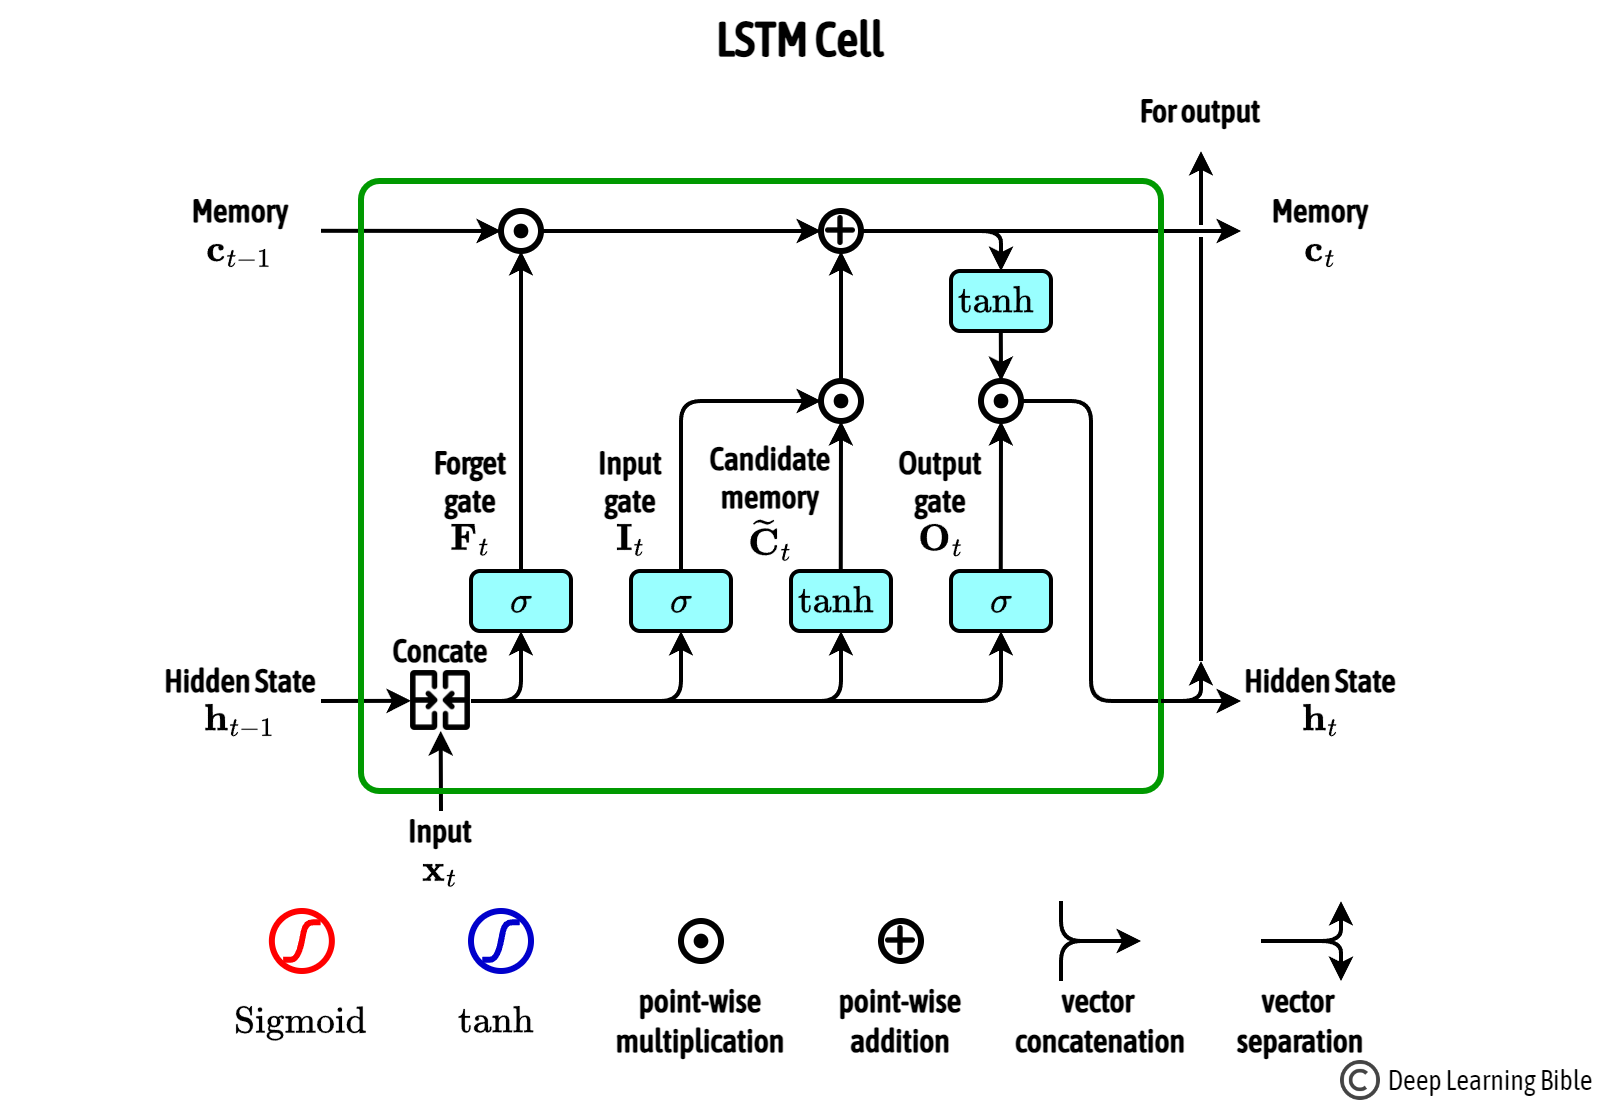
\includegraphics[width=0.5\linewidth]{img/RNN/LSTM_2.png}
    \caption{LSTM cell}
    \label{fig:lstm}
\end{figure}

LSTM cells are organized as follows:
\begin{itemize}
    \item \textbf{Forget gate}: decides which information from long term memory
          be kept or discarded and this is done by multiplying the incoming long
          term memory by a forget vector generated by the current input and
          incoming short memory:
          \begin{equation*}
              f_t = \sigma(W_f \cdot [h^{(t - 1)}, x^{(t)}] + b_f)
          \end{equation*}
    \item \textbf{Input gate}: decides what information will be stored in long
          term memory. It only works with the information from the current input
          and short term memory from the previous step. At this gate, it filters
          out the information from variables that are not useful. First, determine
          which entries in the cell state to update by computing $0 - 1$ sigmoid
          output:
          \begin{equation*}
              i^{(t)} = \sigma(W_i \cdot [h^{(t - 1)}, x^{(t)}] + b_i)
          \end{equation*}
          Then determine what amount to add/subtract from these entries by computing
          a tanh output (valued $-1$ to $1$) function of the input and hidden state:
          \begin{equation*}
              \tilde{C}^{(t)} = \tanh(W_c \cdot [h^{(t - 1)}, x^{(t)}] + b_c)
          \end{equation*}
    \item \textbf{Output gate}: will take the current input, the previous short
          term memory and newly computed long term memory to produce new short
          term memory which will be passed on to the cell in the next time step.
          Hidden state is updated based on a \textit{filtered} version of the
          cell state, scaled to $- 1$ to $1$ using tanh. Output gate computes a
          sigmoid function of the input and previous hidden state to determine
          which elements of the cell state to output:
          \begin{equation*}
              h^{(t)} = \sigma(W_o \cdot [h^{(t - 1)}, x^{(t)}] + b_o) \cdot \tanh C^{(t)}
          \end{equation*}
\end{itemize}

The previous state is multiplied by the forget gate and then added to the fraction
of the new candidate allowed by the input gate:
\begin{equation}
    C^{(t)} = f^{(t)} \cdot C^{(t - 1)} + i^{(t)} \cdot \tilde{C}^{(t)}
\end{equation}

\begin{figure}[!ht]
    \centering
    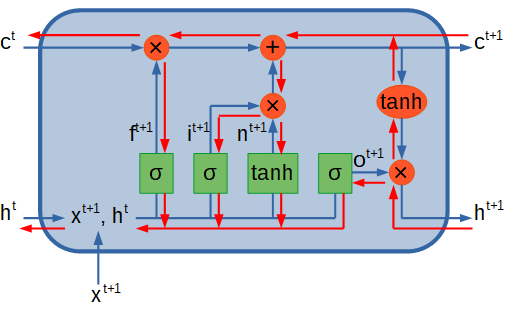
\includegraphics[width=0.45\linewidth]{img/RNN/backprop.png}
    \caption{Backpropagation through time with uninterrupted gradient flow}
    \label{fig:RNNBack}
\end{figure}
\subsection{GRU}
To solve the problem faced by standard RNN, GRU incorporates the two gate operating
mechanisms called \textbf{Update gate} and \textbf{Reset gate}. In particular,
it uses fewer gates than LSTM by combining forget and input gates into update gates
and eliminates cell state vector. This architecture has significant less number
of parameters so it is faster than the other.

\begin{figure}[!ht]
    \centering
    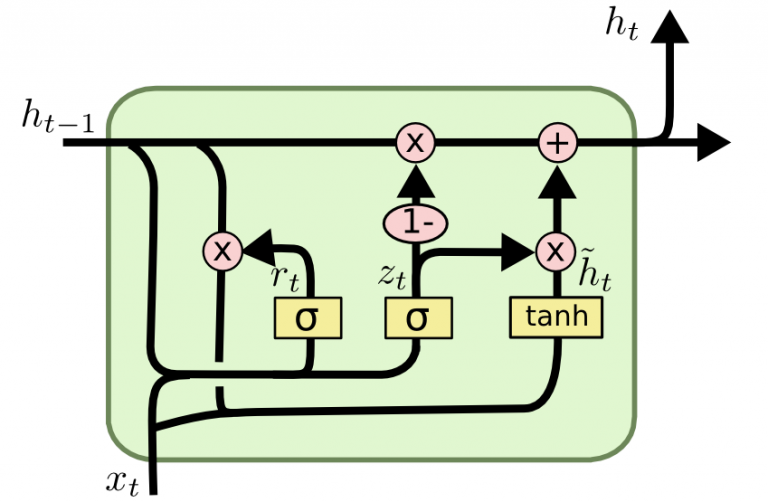
\includegraphics[width=0.45\linewidth]{img/RNN/GRU.png}
    \caption{GRU cell}
    \label{fig:gru}
\end{figure}

GRU cells are organized as follows:
\begin{itemize}
    \item \textbf{Update Gate}: is responsible for determining the amount of previous
          information that needs to pass along the next state. This is really
          powerful because the model can decide to copy all the information from
          the past and eliminate the risk of vanishing gradient;
    \item \textbf{Reset Gate}: it stores relevant information from the past time
          step into new memory content. Then it multiplies the input vector and
          hidden state with their weights. Next, it calculates element-wise
          multiplication between the reset gate and previously hidden state
          multiple. After summing up the above steps the non-linear activation
          function is applied and the next sequence is generated.
\end{itemize}